\section{Condition monitoring}
All rotating machinery eventually fails because of the long-term strain on the individual parts, incorrect workmanship, installation, or operational procedures. In the end, these factors cause the equipment not to fulfill its intended functionality. Many instrumentation methods are practiced to reveal evolving faults: vibration and acoustic noise monitoring, electric supply line measurements, thermography, oil and particle analysis, ultrasonic testing, etc. However, vibration signals are the preferred tool for rotating machinery monitoring \cite{mohanty_machinery_2015}.

The defect needs to be either repaired or replaced, preferably without significant production downtime, further damage to the other attached elements, or any endangerment of the responsible personnel. The maintenance strategies are chosen according to the machine's importance as a result of its failure effect evaluation on the system. The guide to set appropriate maintenance procedures is outlined in the IEC~60706-2 standard and involves reliability-centered maintenance analysis~\cite{el-thalji_predictive_2019}.

\subsection{Maintenance strategies}
There are three different approaches to maintenance across the industry: \textbf{reactive, preventive, and predictive}~\cite{scheffer_practical_2004}. In general, the more sophisticated methods are beneficial in a high-stakes environment. The unexpected machine shutdown can have a negative economic impact on the enterprise, resulting in decreased product quality and demands spare parts to be ready in the supply inventory at all times. In certain situations it suffice to utilize a simpler maintenance program, but the predictive maintenance gains attraction in the Industry 4.0 to optimize assets' usage~\cite{cinar_machine_2020}.
\bigbreak

\textbf{Reactive maintenance} allows machinery to run until a complete failure. This is the most inappropriate way to maintain the production line, but it is straightforward enough. It requires a large stock of replacement parts on-site and breakage inflicts a `crisis management mode' upon the plant \cite{scheffer_practical_2004}. On-demand repairs are justified if short downtime is acceptable, full and swift replacement of a broken machine with a backup is possible, or there is negligable threat to the surrounding environment on failure~\cite{ziaran_technicka_2013}.
\bigbreak

\textbf{Preventive maintenance} is performed before any issue is detected. Maintenance occurs at regular intervals derived from a predetermined period in the calendar or expected machine running time (e.g. MTTF - Mean Time To Failure). The schedule is crucial but can result in components being replaced in good condition creating waste. Occasionally parts can stay in operation too long and as a result the machine breaks. However, conservative planning is usually the norm to keep the machine always in a perfect state and therefore more frequent interventions are required~\cite{mohanty_machinery_2015}.
\bigbreak

\textbf{Predictive maintenance} known as condition-based maintenance (CbM), improves the predictability of reactive maintenance and eliminates the waste in overall resource utilization of cautious prevention. The machine downtime is scheduled after the detection of unhealthy trends in fault monitoring with sensors and troublesome components are identified.

A measurable decrease in effectivity allows us to order necessary parts in advance and organize repairs of several machines at a convenient time. The misdetection leads to increased costs compared to previous methods and raises the expectation that faults are distinguishable among themselves~\cite{davies_handbook_2012}.
\bigbreak

\begin{figure}[h]
	\centering
	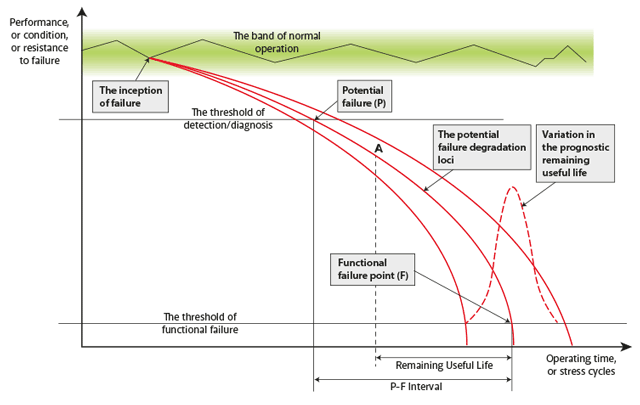
\includegraphics[width=\textwidth]{assets/P-F-Curve.png}
	\caption{P-F curve represents the evolution of the asset's health~\cite{jennions_integrated_2011}}
	\label{fig:p-f-curve}
\end{figure}

The P-F curve is a widespread representation of equipment degradation over time based on historical records (Fig.~\ref{fig:p-f-curve}). Corrective action should be taken between the event of potential failure (P), when the fault detection is activated, and functional failure point (F) in the P-F interval~\cite{bousdekis_enterprise_2021}.  These division points are not exactly set but have statistical distribution to them.

The Remaining Useful Life (RUL) of the specific running machine in the given instance can be merely estimated analytically, with the survival probabilities of the individual components, and based on the model of the `run-to-failure' histories and usage parameters~\cite{okoh_overview_2014}. Predictive condition monitoring aims to extend the machine lifespan to the maximum by predicting expected RUL.

\begin{figure}[h]
	\centering
	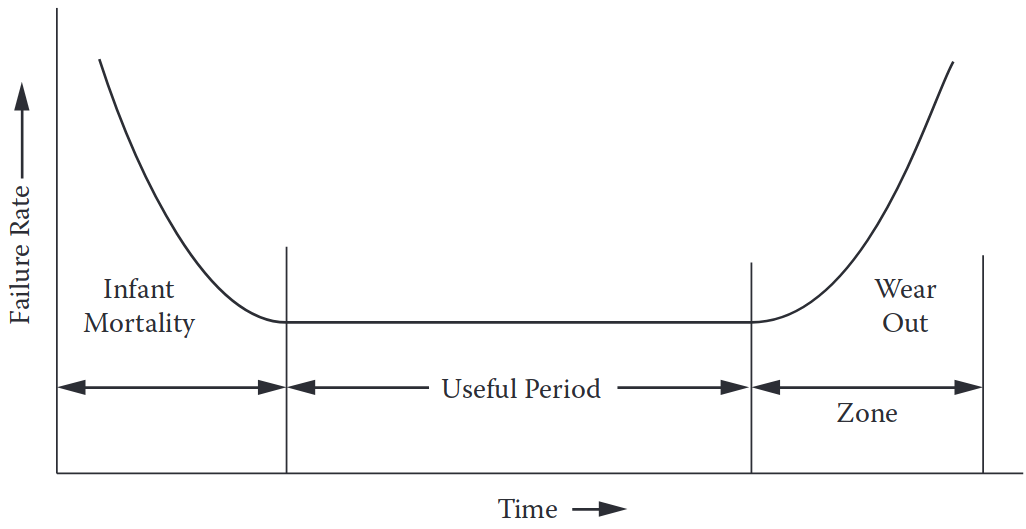
\includegraphics[width=0.8\textwidth]{assets/bath-tub-curve.png}
	\caption{Bath tub curve~\cite{mohanty_machinery_2015}}
	\label{fig:bath-tub-curve}
\end{figure}

A high failure rate is present not only at the worn-out stage when the parts are fatigued or corroded but also in the early stages soon after assembly. Causes can be found in manufacturing or material defects, inadequate installation, or improper start-up procedures. During the stable middle phase, malfunction can occur after the machine's excessive overload. The time plot to failure rate is known as the bath tub curve~(Fig.~\ref{fig:bath-tub-curve}).

\subsection{Vibration fault types}
Mechanical problems during machinery operation bring about vibrations in the vast majority of cases. Therefore vibroacoustic diagnostics is considered one of the most important methods in early component fault identification~\cite{ziaran_technicka_2013}.

The cause of vibration comes out of the changing force in its magnitude or direction. The most emerging defects can be encompassed by explaining the deficiencies of the mechanical structure broadly categorized as \textbf{unbalance, misalignment, looseness, excentricity, deformation, crack and influence of the external force} (e.g. friction)~\cite{davies_handbook_2012}. It is important to stress that our concern are not the underlying deficiencies in mechanical parts, but the correct fault classification based on the signal waveform.

\begin{figure}[h]
	\centering
	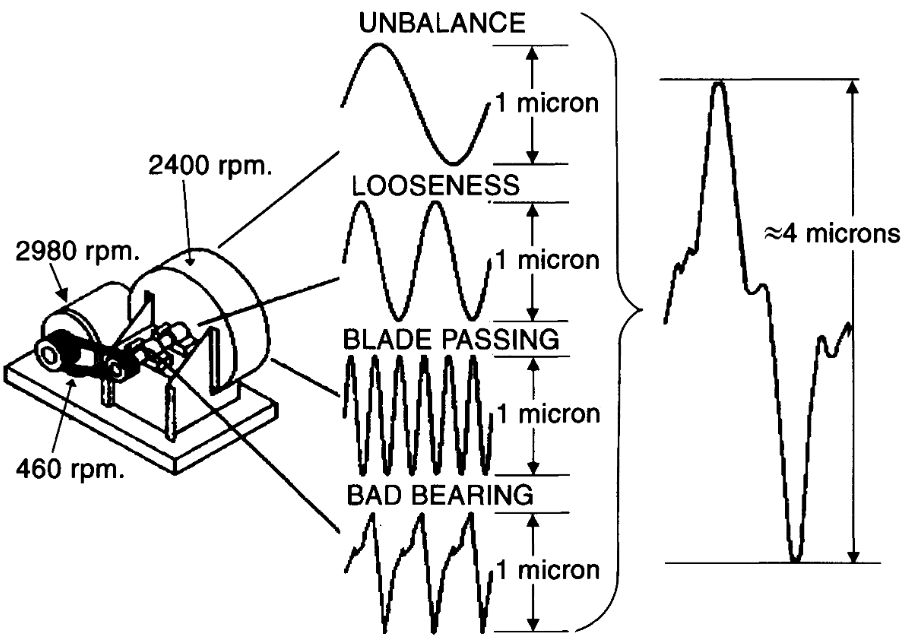
\includegraphics[width=0.6\textwidth]{assets/complex-vibrations.png}
	\caption{Complex machinery vibrations~\cite{davies_handbook_2012}}
	\label{fig:machinery-vibrations}
\end{figure}

Rotating machine disorders do exhibit frequency signatures at various ranges in the frequency spectrum with supplementary symptoms carried in phase. Most of the occurring faults can be tied to the main rotational speed of the component under investigation (Fig.~\ref{fig:machinery-vibrations})~\cite{davies_handbook_2012}. Imbalance, misalignment, and looseness normally appear at frequencies up to 300 Hz. These low-frequency faults are associated with the movement of the shaft and primarily coincide with revolution speed and its harmonics. Bearing and gearbox defects in the late stages of development, show up in the range between 300 Hz to 1 kHz. Higher frequencies, measured traditionally to a limit of 10 kHz, help notice the deficiencies in bearings even sooner~\cite{torres_automatic_2022}.

One of the methods vibration experts utilize in the identification of the damaged part from the frequency spectrum is \textbf{order analysis}. In essence, it is about noticing the excessive peaks at harmonic frequencies that are integer multiples of fundamental frequency (1x rpm)~(Tab.~\ref{tab:vibration-causes}):

\begin{table}[h]
\renewcommand{\arraystretch}{1.2}
\begin{adjustbox}{width=\columnwidth,center}
\begin{tabular}{|ll|l|l|}
\hline
\multicolumn{2}{|l|}{\textbf{Frequency content}}                            & \textbf{Likely reason}                                                                                                     & \textbf{Other causes}                                                                                                                          \\ \hline
\multicolumn{1}{|l|}{\multirow{4}{*}{Synchronous}} & 1 x rpm                & Imbalance                                                                                                                & \begin{tabular}[c]{@{}l@{}}Eccentric journals\\ Bent shaft / Misalignment\\    (high axial vibration)\\ Bad belt (if rpm of belt)\end{tabular} \\ \cline{2-4}
\multicolumn{1}{|l|}{}                             & 2 x rpm                & Looseness                                                                                                                & \begin{tabular}[c]{@{}l@{}}Misalignment \\    (high axial vibration)\\ Cracked rotor\\ Bad belt (if rpm of belt)\end{tabular}                  \\ \cline{2-4}
\multicolumn{1}{|l|}{}                             & 3 x rpm                & Misalignment                                                                                                             & and axial looseness                                                                                                                             \\ \cline{2-4}
\multicolumn{1}{|l|}{}                             & Many x rpm             & \begin{tabular}[c]{@{}l@{}}Bad gears\\ Severe looseness\end{tabular}                                                     & \begin{tabular}[c]{@{}l@{}}Gear teeth x rpm\\ Fan blade count x rpm\end{tabular}                                                               \\ \hline
\multicolumn{1}{|l|}{Sub-synchronous}                 & \textless 1 x rpm      & Oil whirl                                                                                                                & \begin{tabular}[c]{@{}l@{}}Bad drive belt\\ Background\\ Resonance\end{tabular}                                                                \\ \hline
\multicolumn{1}{|l|}{Non-synchronous}              & \multicolumn{1}{c|}{-} & \begin{tabular}[c]{@{}l@{}}Electrical problems (x 50 Hz)\\ Reciprocating forces\\ Aerodynamic forces \\ Bad antifriction bearings\end{tabular} & Rubbing \\ \hline
\end{tabular}
\end{adjustbox}
\caption{Expert observed likely vibration causes (based on~\cite{davies_handbook_2012,ziaran_technicka_2013,noauthor_iso_2002})}
\label{tab:vibration-causes}
\end{table}

Because of inherent tolerances in machine manufacturing and assembly, the rotational frequency always manifests itself, even in baseline signature~\cite{davies_handbook_2012, noauthor_iso_2002}. In the most likely scenario, some faults appear as compared to rotational frequency solely in \textbf{synchronous, subsynchronous, or non-synchronous components}. The defects can occur also in a predictable combination of the ones mentioned. Other common patterns experts look for are modulation sidebands typical for bearings and gears extractable with cepstrum analysis~\cite{ziaran_technicka_2013}. Therefore procedure relying on elimination narrows down unrelated causes effectively.

\subsection{Technical standards}
Vibration-based condition monitoring practices adopted in the factory's predictive maintenance management must comply with normative guidelines formalized in ISO international standards. The standards are concerned with each step in the process that originates with transducer placements and data acquisition. They prescribe conventions for setting fault severity levels and provide empirically observed vibration characteristics of common defects. Two relevant standards for IoT diagnostics systems are \emph{ISO 20816} (updated from ISO 10816) and \emph{ISO 13373}.
\bigbreak

\textbf{ISO 20816-1:2016} establishes the approach to vibration measurement and evaluation on non-rotating housing of machinery parts~\cite{noauthor_iso_2016}. The measurement units are agreed upon for kinematic quantities of vibrations. Acceleration is to be measured in meters per second squared ($m/s^2$), velocity in millimeters per second ($mm/s$), and displacement in micrometers ($\mu m$). It is customary to evaluate broad-band vibration velocity in terms of root mean square value (RMS), as it has a relation to its signal energy. No simple direct relationship is expressible among these quantities, except in stationary signals.

The vibration severity is the maximum magnitude value measured in two radial directions (horizontal, and vertical) or supplemented with a third direction along the shaft in the axial axis. Multiple measurement locations, i.e. on several bearings or couplings, should be assessed independently.

Criteria introduced to judge vibration severity are its absolute vibration magnitude, change in the magnitude vector, and rate of change. In terms of maximal magnitudes the machines of varied sizes are split into four severity zones defined in the chart ~(Tab.~\ref{tab:iso20816-vibration-severity}). The table values serve as guidelines towards realistic requirements between machine manufacturers and customers.

\begin{table}[h]
\centering
\renewcommand{\arraystretch}{1.2}
\begin{adjustbox}{width=\columnwidth,center}
\begin{tabular}{|c|c|c|c|c|}
\hline
\textbf{\begin{tabular}[c]{@{}c@{}}Vibration velocity\\ RMS {[}mm/s{]}\end{tabular}} & \textbf{\begin{tabular}[c]{@{}c@{}}Class I\\ Small machines\end{tabular}} & \textbf{\begin{tabular}[c]{@{}c@{}}Class II\\ Medium machines\end{tabular}} & \textbf{\begin{tabular}[c]{@{}c@{}}Class III\\ Large machines\\ Rigid supports\end{tabular}} & \textbf{\begin{tabular}[c]{@{}c@{}}Class IV\\ Large machines\\ Flexible support\end{tabular}} \\ \hline
0.28                                                                                 & \cellcolor[HTML]{9AFF99}                                                  & \cellcolor[HTML]{9AFF99}                                                    & \cellcolor[HTML]{9AFF99}                                                                     & \cellcolor[HTML]{9AFF99}                                                                      \\ \cline{1-1}
0.45                                                                                 & \cellcolor[HTML]{9AFF99}                                                  & \cellcolor[HTML]{9AFF99}                                                    & \cellcolor[HTML]{9AFF99}                                                                     & \cellcolor[HTML]{9AFF99}                                                                      \\ \cline{1-1}
0.71                                                                                 & \multirow{-3}{*}{\cellcolor[HTML]{9AFF99}\textbf{Good (A)}}               & \cellcolor[HTML]{9AFF99}                                                    & \cellcolor[HTML]{9AFF99}                                                                     & \cellcolor[HTML]{9AFF99}                                                                      \\ \cline{1-2}
1.12                                                                                 & \cellcolor[HTML]{FFFC9E}                                                  & \multirow{-4}{*}{\cellcolor[HTML]{9AFF99}\textbf{Good (A)}}                 & \cellcolor[HTML]{9AFF99}                                                                     & \cellcolor[HTML]{9AFF99}                                                                      \\ \cline{1-1} \cline{3-3}
1.8                                                                                  & \multirow{-2}{*}{\cellcolor[HTML]{FFFC9E}\textbf{Satisfactory (B)}}       & \cellcolor[HTML]{FFFC9E}                                                    & \multirow{-5}{*}{\cellcolor[HTML]{9AFF99}\textbf{Good (A)}}                                  & \cellcolor[HTML]{9AFF99}                                                                      \\ \cline{1-2} \cline{4-4}
2.8                                                                                  & \cellcolor[HTML]{F8A102}                                                  & \multirow{-2}{*}{\cellcolor[HTML]{FFFC9E}\textbf{Satisfactory (B)}}         & \cellcolor[HTML]{FFFC9E}                                                                     & \multirow{-6}{*}{\cellcolor[HTML]{9AFF99}\textbf{Good (A)}}                                   \\ \cline{1-1} \cline{3-3} \cline{5-5}
4.5                                                                                  & \multirow{-2}{*}{\cellcolor[HTML]{F8A102}\textbf{Unsatisfactory (C)}}     & \cellcolor[HTML]{F8A102}                                                    & \multirow{-2}{*}{\cellcolor[HTML]{FFFC9E}\textbf{Satisfactory (B)}}                          & \cellcolor[HTML]{FFFC9E}                                                                      \\ \cline{1-2} \cline{4-4}
7.1                                                                                  & \cellcolor[HTML]{FD6864}                                                  & \multirow{-2}{*}{\cellcolor[HTML]{F8A102}\textbf{Unsatisfactory (C)}}       & \cellcolor[HTML]{F8A102}                                                                     & \multirow{-2}{*}{\cellcolor[HTML]{FFFC9E}\textbf{Satisfactory (B)}}                           \\ \cline{1-1} \cline{3-3} \cline{5-5}
11.2                                                                                 & \cellcolor[HTML]{FD6864}                                                  & \cellcolor[HTML]{FD6864}                                                    & \multirow{-2}{*}{\cellcolor[HTML]{F8A102}\textbf{Unsatisfactory (C)}}                        & \cellcolor[HTML]{F8A102}                                                                      \\ \cline{1-1} \cline{4-4}
18                                                                                   & \cellcolor[HTML]{FD6864}                                                  & \cellcolor[HTML]{FD6864}                                                    & \cellcolor[HTML]{FD6864}                                                                     & \multirow{-2}{*}{\cellcolor[HTML]{F8A102}\textbf{Unsatisfactory (C)}}                         \\ \cline{1-1} \cline{5-5}
28                                                                                   & \cellcolor[HTML]{FD6864}                                                  & \cellcolor[HTML]{FD6864}                                                    & \cellcolor[HTML]{FD6864}                                                                     & \cellcolor[HTML]{FD6864}                                                                      \\ \cline{1-1}
45                                                                                   & \multirow{-5}{*}{\cellcolor[HTML]{FD6864}\textbf{Unacceptable (D)}}       & \multirow{-4}{*}{\cellcolor[HTML]{FD6864}\textbf{Unacceptable (D)}}         & \multirow{-3}{*}{\cellcolor[HTML]{FD6864}\textbf{Unacceptable (D)}}                          & \multirow{-2}{*}{\cellcolor[HTML]{FD6864}\textbf{Unacceptable (D)}}                           \\ \hline
\end{tabular}
\end{adjustbox}
\caption{ISO 20816 vibration severity chart with typical magnitudes \cite{noauthor_iso_2016}}
\label{tab:iso20816-vibration-severity}
\end{table}

\emph{Zone A} is reserved for newly commissioned machines. \emph{Zone B} signifies suitability for long-term operation. In \emph{zone C} is the machine deemed in unsatisfactory condition and corrective action should be taken soon. Finally, in zone D vibrations can cause damage to the machine. The span of acceptable values differs on machine class from I through to IV with an output power of 15~kW (class~I), 75~kW (class~II), 10~MW (class~III), or greater.

The operational limits in the form of \emph{alarms} and \emph{trips} are usually established on the zone boundaries or close to them. Alarms are placed between zones B and C and provide a warning about reaching the threshold significant for noticeable change. Trips in between zones C and D urge immediate action or machine shut down. Both limits should not exceed 1.25 times the upper boundary or lower zones and initially are set based on previous experience with the machine~\cite{noauthor_iso_2002}.

\textbf{ISO 13373-1:2002} delves into further nuances of vibration monitoring and expands on procedures outlined in the vocabulary of ISO 20186. According to the standard, the data collection operates in continuous or periodic observation modes which follow an event or intervals. Both designs can be permanently mounted, but in continuous, collection `multiplexing rate is sufficiently rapid so there is no significant data or trends lost'~\cite{noauthor_iso_2002}.  When channels are scanned successively with gaps between data points the system is known as `scanning'.

The condition monitoring programme is run according to a flowchart adapted from one designed in the standard specifically to best benefit the plant. Those steps can be summarized as follows~\cite{noauthor_iso_2002}:
\begin{enumerate}
\itemsep0pt
\item Review machinery history and establish failure modes.
\item When vibration monitoring is not applicable check for other condition monitoring techniques or resort to preventive maintenance.
\item Select monitoring points and take preliminary vibration measurements.
\item Select vibration monitoring techniques: broadband, frequency analysis, or special techniques, and set parameters of measurement units.
\item Take baseline measurements.
\item Change levels that would warrant investigation.
\item Carry out routine condition monitoring.
\item If an alarm was exceeded, notify appropriate personnel to review data and trends, perform diagnostic evaluation, and repair as necessary. In case a new baseline is needed continue in the step of taking baseline measurements.
\item Shut down the machine when the trip level is exceeded. Then proceed the same as after the alarm trigger.
\end{enumerate}

Measurement of vibrations should be accompanied by a description of the machine and its operating conditions. The machine description includes the machine identifier and its type, power source, rated rotation speed and power, configuration (shaft or belt driven), and machine support. Measurement parameters such as timestamp, transducer type, sensor location and orientation in MIMOSA code, measurement units and units qualifier (p-p, RMS), and other processing options (filters, number of averages, etc.) are to be recorded alongside the measurement value itself~\cite{noauthor_iso_2002}.

The transducer of choice for condition monitoring is the accelerometer which can provide the acceleration value of the body and velocity after signal integration. However, standard cautions against double integrating for displacement. The recommended frequency range for an accelerometer is 0.1~Hz to 30~kHz. The choice of transducer mount significantly lowers its resonance frequency which is least influenced by stud mount and stiff cement mount. The resonance is reduced to around 8~kHz with the use of soft epoxy or permanent magnet.

\begin{figure}[h]
	\centering
	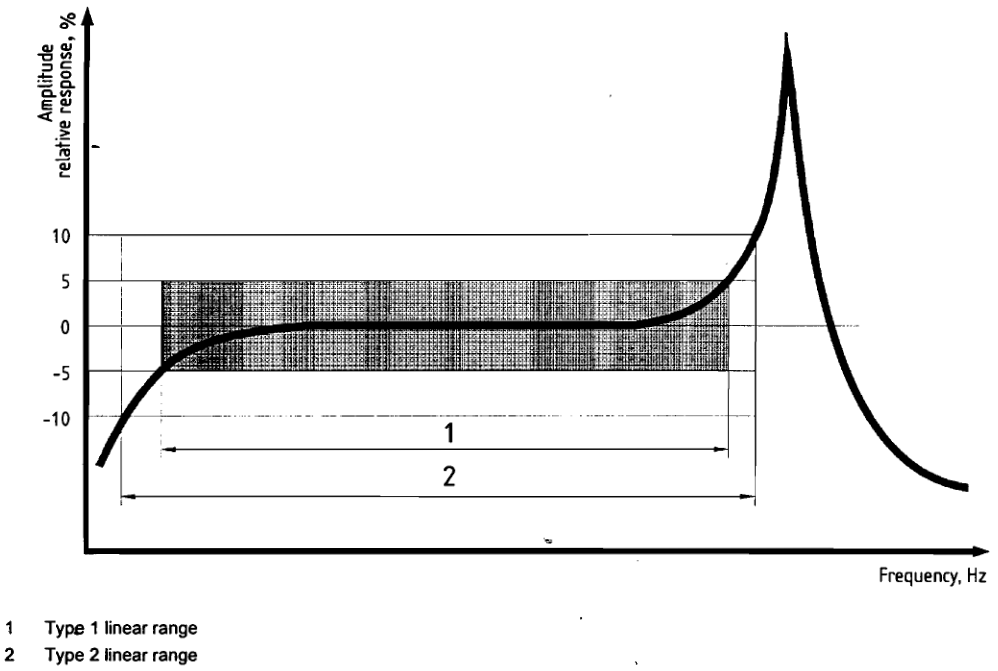
\includegraphics[width=0.8\textwidth]{assets/transducer-response.png}
	\caption{The transducer linear response and resonance in tolerance intervals~\cite{noauthor_iso_2002}}
	\label{fig:tranducer-response}
\end{figure}

Broadband measurement requires `frequency ranges of 0.2 times the lowest rotational frequency to the highest frequency of interest'~\cite{noauthor_iso_2002}, not exceeding 10 kHz, with RMS velocity 0.1 - 100~mm/s. Bearings and gears diagnosis may push the upper-frequency limit even higher. The tolerances of amplitude and frequency calibrations fall into two types with allowable tolerances of $\pm 5 \%$ or $\pm 10 \%$~(Fig.~\ref{fig:tranducer-response}).

Equipment's `health' can be mischaracterized when there are significant differences in the machine's normal operating conditions. Baseline measurements in all acceptable conditions are to be acquired to reduce the error in vibration evaluation. According to bath tub curve~(Fig.~\ref{fig:bath-tub-curve}) reference signatures should be obtained after the initial part wear-in period. The reference spectral mask of the baseline condition is designed if maximal acceptance amplitudes are different for each significant frequency band ~\cite{ziaran_technicka_2013}.

The vibration baseline is defined by broad-band magnitudes and phases of motion vectors, waveforms in time and frequency domain, the rotational speed of the machine as well as its frequency response to different speeds during start-up and coast-down captured in the Bode plot and waterfall plot. Changes during the machine operation are then depicted in value trends. Trends can be shown of overall amplitudes or limited to frequency bands.
